%
% problemstellung.tex -- Grundlagen ueber Differentialgleichungen
%
% (c) 2015 Prof Dr Andreas Mueller, Hochschule Rapperswil
%
\section{Problemstellung
\label{buch:section:dglproblemstellung}}
\rhead{Differentialgleichungen}
Eine gewöhnliche Differentialgleichung für eine reellwertige
\index{Differentialgleichung}
Funktion $y(x)$ stellt einen Zusammenhang her zwischen der Funktion
und ihren Ableitungen.
Wir schreiben die Ableitungen als $y'$, $y''$, $y'''$ und $y^{(n)}$
für die $n$-te Ableitung.
Wir lassen oft das Argument der Funktion weg.
Beispiele von Differentialgleichungen sind
\begin{align*}
y'&=-Ny
&&\text{Ordnung: $1$}
\\
y''&=-\omega^2 y
&&\text{Ordnung: $2$}
\\
x^2y''+xy'+(x^2-n^2)y&=0
&&\text{Ordnung: $2$}
\end{align*}
Die Abhängigkeit kann in expliziter Form als
\index{Differentialgleichung!explizite Form}%
\index{explizite Form einer Differentialgleichung}%
\begin{equation}
y^{(n)}=f(x,y,y',\dots,y^{(n-1)})
\label{grundlagen:explizit}
\end{equation}
oder in impliziter Form
\index{Differentialgleichung!implizite Form}%
\index{implizite Form einer Differentialgleichung}%
\[
F(x,y,y',\dots,y^{(n)})=0
\]
gegeben sein.
Die Ordnung einer Differentialgleichung ist die höchste vorkommende
Ableitung.
\index{Ordnung!einer Differentialgleichung}%

\begin{figure}
\centering
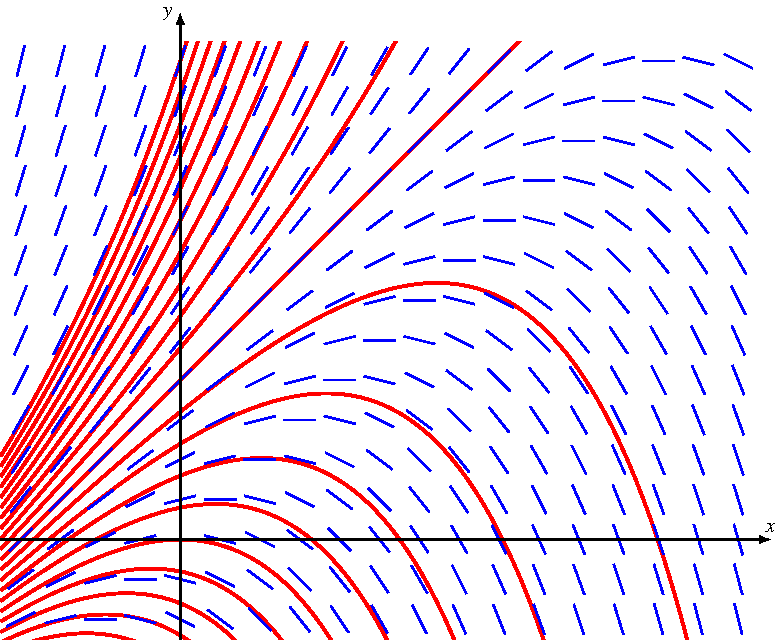
\includegraphics{chapters/50-ode/figures/grundlagen.pdf}
\caption{Richtungsfeld der Differentialgleichung $y'=y-x$ mit
einzelnen Lösungskurven.
\label{grundlagen:richtungsfeld}}
\end{figure}%

Differentialgleichungen erster Ordnung lassen sich mit Hilfe eines
Richtungsfeldes visualisieren, wie in Abbildung~\ref{grundlagen:richtungsfeld}
dargestellt.
\index{Richtungsfeld}%
In jedem Punkt $(x,y)$ der $x$-$y$-Ebene wird die Steigung $y'=f(x,y)$
eingezeichnet.
Eine Lösung der Differentialgleichung hat in diesem Bild als Graph
eine Kurve in der $x$-$y$-Ebene, die an jeder Stelle als Tangente 
das Richtungsfeld haben.

Insbesondere in Anwendungen in der Physik ist die Zeit die
unabhängige Variable.
Die abhängige Variable ist dann zum Beispiel die Ortskoordinate
$x(t)$ und wir bezeichnen ihre Ableitungen mit $\dot{x}(t)$ für
die Geschwindigkeit, $\ddot{x}(t)$ für die Beschleunigung.
Dieses Beispiel suggeriert auch, dass die abhängige Variable 
ein Vektor sein kann, den man als den Ortsvektor eines Teilchens
interpretieren kann.
Auch die Funktion $f(t,x,\dots,x^{(n-1)})$ muss dann vektorwertig sein, und
ebenso alle Argumente ausser dem ersten von $f$.

\subsection{Reduktion der Ordnung}
\index{Reduktion der Ordnung}%
\index{Ordnung!Reduktion der}%
Eine Differentialgleichung $n$-ter Ordnung für eine skalare Funktion
kann in eine Vektor-Differen\-tialgleichung erster Ordnung für eine
\index{Vektor-Differentialgleichung}%
\index{Differentialgleichung!Vektor-}%
$n$-dimensionale vektorwertige Funktion umgewandelt werden.
Ist $y(x)$ die gesuchte Funktion in der
Differentialgleichung~\eqref{grundlagen:explizit}, dann kann man
den Vektor
\[
u(x)=\begin{pmatrix}
y(x)\\y'(x)\\\vdots\\y^{(n-1)}(x)
\end{pmatrix}
\in\mathbb R^n
\]
bilden.
Er erfüllt die Differentialgleichung
\begin{equation}
\frac{d}{dx}\begin{pmatrix}
y\\y'\\\vdots\\y^{(n-1)}
\end{pmatrix}
=
\begin{pmatrix}
y'\\y''\\\vdots\\y^{(n)}
\end{pmatrix}
=
\begin{pmatrix}
y'\\y''\\\vdots\\f(x,y,y',\dots,y^{(n-1)})
\end{pmatrix}.
\label{grundlagen:vektordgl}
\end{equation}
Der Vektor auf der rechten Seite hängt nur von $x$, der Funktion $y$
und ihren Ableitungen bis zur $n-1$-ten Ordnung ab, also von $u$, man
kann \eqref{grundlagen:vektordgl} daher als
\begin{equation}
\frac{d}{dx}u=\tilde{f}(x,u)
\end{equation}
schreiben.
Im Folgenden werden wir fast ausschliesslich Differentialgleichungen
erster Ordnung der Form $y'=f(x,y)$ betrachten, und dabei stillschweigend
zulassen, dass $y$ ein Vektor ist.

\subsection{Anfangswertprobleme\label{section:anfangswertprobleme}}
\index{Anfangswertproblem}%
Die Differentialgleichung $y'=f(x,y)$ alleine kann eine Lösungsfunktion
$y(x)$ nicht festlegen, sie codiert nur, wie sich die Lösung verändern wird.
Es ist also zusätzlich die Angabe eines Punktes der Lösungskurve
notwendig.
Man nennt das Problem, eine Funktion $y(x)$ zu finden, welche
\[
y'=f(x,y)
\qquad
\text{und}
\qquad
y(0)=y_0
\]
erfüllt, ein {\em Anfangswertproblem}.
Ein Anfangswertproblem verlangt für die gewöhnliche Differentialgleichung
$n$-ter Ordnung verlangt also die Angabe der Werte von
$y(0),y'(0),\dots,y^{(n-1)}(0)$

\subsubsection{Existenz und Eindeutigkeit von Lösungen}
Die Existenz und Eindeutigkeit einer Lösung ist aus den Beispielen und
graphischen Darstellungen intuitiv verständlich, für einen exakten
Beweis sind jedoch zusätzliche Voraussetzungen nötig.

\begin{definition}
Eine Funktion $f\colon \mathbb R^n\to\mathbb R^m$ heisst global
{\em Lipschitz-stetig},
\index{Lipschitz-stetig}%
wenn es eine Zahl $L$ gibt 
\begin{equation}
|f(x_2)-f(x_1)| \le L\,|x_2-x_1|
\label{grundlagen:lipschitz}
\end{equation}
für alle Vektoren $x_1,x_2\in\mathbb R^n$.
Eine Funktion heisst lokal Lipschitz-stetig im Punkt $x_0$, wenn die
Bedingung \eqref{grundlagen:lipschitz} für $x_i$ in einer Umgebung von
$x_0$ erfüllt ist.
\end{definition}

Eine Funktion ist insbesondere dann lokal Lipschitz-stetig, wenn sie
stetig differenzierbar ist.
In diesem Fall ist die Ableitung $f'(x)$ in einer Umgebung von $x_0$
beschränkt, also $|f(x)|<M$, und der Mittelwertsatz der Differentialgleichung
sagt, dass
\[
|f(x_2)-f(x_1)|\le M |x_2-x_2|
\]
ist, $f$ ist also lokal Lipschitz-stetig.

\begin{satz}[Picard-Lindelöf]
\label{grundlagen:picard-lindeloef}
\index{Satz von Picard-Lindelof@Satz von Picard-Lindel\öf}%
\index{Picard-Lindelof@Picard-Lindel\öf, Satz von}%
Ist die Funktion $f(x,y)$ lokal Lipschitz-stetig bezüglich der Variablen
$y$ für $x\in[x_0,b]$ und $|y-y_0|<R$.
Dann hat das Anfangswertproblem
\[
y'(x)=f(x,y)\qquad\text{und}\qquad y(x_0)=y_0
\]
ein eindeutige Lösung, die in einem Intervall $[x_0,x_0+\varepsilon)$
definiert ist.
\end{satz}
\index{Existenz}%
\index{Eindeutigkeit}%

In diesem Buch werden die Funktionen $f$ der Differentialgleichungen 
meistens stetig differenzierbar sein, so dass der
Satz~\ref{grundlagen:picard-lindeloef} in unseren Anwendungen die lokale
Existenz und Eindeutigkeit einer Lösung garantiert.

\subsection{Randwertprobleme\label{section:randwertprobleme}}
Wenn man einen Ball wirft, wird seine Bewegung durch die
Vektordifferentialgleichung zweiter Ordnung
\[
\frac{d^2}{dt^2}\begin{pmatrix}x\\y\end{pmatrix}
=
\begin{pmatrix}0\\\displaystyle-\frac{g}{m}\end{pmatrix}
\]
beschrieben.
Die Bahn ist ausserdem bestimmt durch die Anfangsbedingungen,
d.~h.~den Anfangspunkt und die Anfangsgeschwindigkeit der Bahn.
Praktischer Ballwurf verlangt aber, dass ein Ziel getroffen wird.
Die Aufgabenstellung ist daher eine Bahnkurve $\gamma(t)$ zu finden,
welche sowohl durch den Anfangspunkt als auch den Zielpunkt
verläuft.

Die Lösung einer Differentialgleichungen erster Ordnung für eine
unbekannte reellwertige Funktion $y(x)$ ist vollständig durch einen
einzigen Anfangswert bestimmt.
Eine Differentialgleichung zweiter Ordnung für eine unbekannte
rellwertige Funktion $y(x)$ verlangt dagegen zwei Anfangswerte,
nämlich für $y(0)$ und $y'(0)$.
In Analogie zum Problem des Ballwurfs könnte die Lösungsfunktion auch
festgelegt werden durch den Wert für $x=0$ und $x=1$.
Gesucht ist also eine Funktion $y(x)$ auf dem Intervall $[0,1]$, die
\begin{equation}
y''=f(x,y,y')
\qquad\text{mit}\qquad
y(0)=y_0,
\qquad
y(1)=y_1
\end{equation}
erfüllt.
Die Lösungsfunktion muss also bestimmte Werte am Rand des Definitionsbereichs
annehmen, man spricht von einem {\em Randwertproblem}.
\index{Randwertproblem}%

\begin{beispiel}
Wir lösen die Differentialgleichung $y''=-y$ mit den Randwerten
$y(0)=1$ und $y(1)=2$.
Die homogene Differentialgleichung hat die Funktionen
\[
y(x)=A \cos x + B\sin x
\]
als allgemeine Lösung.
Die Konstanten $A$ und $B$ müssen so gewählt werden, dass die Randwerte
korrekt sind.
Setzt man $x=0$ und $x=1$ ein, erhält man die linearen Gleichungen
\begin{align*}
a=y(0)&=A\cos 0 + B\sin 0=A\\
b=y(1)&=A\cos 1 + B\sin 1
\qquad\Rightarrow\qquad
\frac{b-a\cos 1}{\sin 1}.
\end{align*}
Die Lösung des Randwertproblems ist daher die Funktion
\[
y(x)=a\cos x +\frac{b-a\cos 1}{\sin 1}\sin x,
\]
wie man auch durch Einsetzen von $x=0$ und $x=1$ verifizieren kann.
\end{beispiel}

\subsection{Höhere Ableitungen\label{grundlagen:hoehere-ableitungen}}
\index{hohere Ableitungen@h\öhere Ableitungen}%
Die Differentialgleichung $y'=f(x,y)$ erlaubt nicht nur die erste
Ableitung einer Funktion zu bestimmen.
Durch Ableitung nach $x$ können wir auch die höheren Ableitungen
bestimmen, die eine Lösung der Differentialgleichung haben muss,
die durch den Punkt $(x,y)$.
\begin{align}
y'(x)
&=
f(x,y),
\notag
\\
y''(x)
&=
\frac{dy'(x)}{dx}
=
\frac{\partial f(x,y)}{\partial x} + \frac{\partial f(x,y)}{\partial y}y'(x)
=
\frac{\partial f(x,y)}{\partial x} + \frac{\partial f(x,y)}{\partial y}f(x,y),
\label{grundlagen:2abl}
\\
y'''(x)
&=
\frac{dy''(x)}{dx}
\notag
\\
&=
\frac{\partial^2 f(x,y)}{\partial x^2}
+ \frac{\partial^2 f(x,y)}{\partial y\,\partial x}y'(x)
+ \biggl(\frac{\partial^2 f(x,y)}{\partial x\,\partial y}
+ \frac{\partial^2 f(x,y)}{\partial y^2}y'(x)\biggr)f(x,y)
\notag
\\
&\qquad
+ \frac{\partial f(x,y)}{\partial y}\biggl(
\frac{\partial f(x,y)}{\partial x} + \frac{\partial f(x,y)}{\partial y}f(x,y)
\biggr),
\notag
\\
&=
\frac{\partial^2 f(x,y)}{\partial x^2}
+ 2\frac{\partial^2 f(x,y)}{\partial x\,\partial y}f(x,y)
+ \frac{\partial^2 f(x,y)}{\partial y^2}f(x,y)^2
+ \biggl(\frac{\partial f(x,y)}{\partial y}\biggr)^2 f(x,y)
+ \frac{\partial f(x,y)}{\partial y} \frac{\partial f(x,y)}{\partial x}.
\label{grundlagen:3abl}
\end{align}
Die Terme werden offensichtlich schnell kompliziert.

\subsection{Ableitung nach der Anfangsbedingung\label{grundlagen:jacobi}}
\index{Ableitung!nach der Anfangsbedingung}%
Verändert man die Anfangsbedingung, ändert sich auch die Lösung,
die Komponente $y_i$ ist also eine Funktion von $x$ und
von allen Anfangswerten $y_{j0}$:
\[
y_i(x, y_{10},\dots,y_{n0}).
\]
Wenn man untersuchen will, wie empfindlich die $y_i$ auf Änderungen
der Anfangswerte reagieren, dann sucht man die Ableitungen der $y_i$
nach den Anfangswerten, also die sogenannte Jacobi-Matrix
\index{Jacobi-Matrix}%
\[
J(x)
=
\begin{pmatrix}
\displaystyle\frac{\partial y_1}{\partial y_{10}}&\dots&
	\displaystyle\frac{\partial y_1}{\partial y_{n0}}\\
\vdots&\ddots&\vdots\\
\displaystyle\frac{\partial y_n}{\partial y_{10}}&\dots&
	\displaystyle\frac{\partial y_n}{\partial y_{n0}}\\
\end{pmatrix}
\]
Wir schreiben abkürzend auch 
\[
J(x)= \frac{\partial y}{\partial y_0}.
\]
Für $x=0$ ist $y(x)=y(0)=y_0$, die Ableitung der $y$-Werte nach den
Anfangswerten ist daher die Einheitsmatrix:
\[
J(0)=E,
\]
und es liegt nahe, dass auch $J(x)$ eine Differentialgleichung erfüllen
muss.

Wie ändert sich $J(x)$ zwischen $x$ und $x+\Delta x$?
Die Werte von $y$ ändern sich um
\begin{equation}
\frac{dy}{dx}= f(x,y),
\label{grundlagen:jacobi-1}
\end{equation}
aber $y$ hängt von den Anfangsbedingungen ab.
Leiten wir \eqref{grundlagen:jacobi-1} nach $y_0$ ab, finden wir
\begin{equation}
\frac{\partial}{\partial y_0}\frac{dy}{dx}
=
\frac{\partial}{\partial y_0}f(x,y).
\label{grundlagen:jacobi-2}
\end{equation}
Die rechte Seite wir mit der Kettenregel zu
\begin{align*}
\frac{\partial}{\partial y_{j0}}f_i(x,y).
&=
\sum_{k=1}^n \frac{\partial f_i(x,y)}{\partial y_{k}}
\underbrace{\frac{\partial y_k}{\partial y_{j0}}}_{\displaystyle J_{ij}(x)}.
\end{align*}
Schreiben wir die Ableitungen von $f$ nach $y$ in die Matrix
\[
\frac{\partial f(x,y)}{\partial y}
=
\begin{pmatrix}
\displaystyle\frac{\partial f_1(x,y)}{\partial y_1}&\dots&
	\displaystyle\frac{\partial f_1(x,y)}{\partial y_n}\\
\vdots&\ddots&\vdots\\
\displaystyle\frac{\partial f_n(x,y)}{\partial y_1}&\dots&
	\displaystyle\frac{\partial f_n(x,y)}{\partial y_n}
\end{pmatrix}
=F(x,y),
\]
kann die Gleichung \eqref{grundlagen:jacobi-2} mit dem Matrizenprodukt als
\begin{equation*}
\frac{\partial}{\partial y_0}\frac{dy}{dx}
=
F(x,y)J(x)
\end{equation*}
sehr viel kompakter geschrieben werden.
Die Ableitungen auf der linken Seite vertauschen, und wir erhalten

\begin{satz}
Ist $y(x,y_0)$ die Lösung der Differentialgleichung 
\[
y'=f(x,y)\qquad\text{mit Anfangsbedingung}\qquad y(0)=y_0,
\]
dann erfüllt die Jacobi-Matrix 
\[
\frac{\partial y}{\partial y_0}=J(x)
\]
die Differentialgleichung
\begin{equation}
\frac{d}{dx}\frac{\partial y}{\partial x}
=
\frac{d}{dx}J(x)
=
F(x,y)J(x)
\qquad
\text{mit Anfangsbedingung}
\qquad
J(x)=E,
\label{grundlagen:jacobi-dgl}
\end{equation}
wobei $F$ die Ableitung von $f$ nach $y$ ist,
\[
F(x,y)=\frac{\partial f(x,y)}{\partial y}.
\]
\end{satz}
Vor allem bei der numerischen Lösung mit dem Computer lässt sich
die Jacobi-Matrix also gleich mit bestimmen, indem man die gefundene
Lösung $y$ als Input für die Gleichung \eqref{grundlagen:jacobi-dgl}
verwendet.

\begin{beispiel}
Wir betrachten wieder die Schwingungsdifferentialgleichung $y''=-y$,
oder vielmehr die Form erster Ordnung
\[
\frac{d}{dx}\begin{pmatrix}y_1\\y_2\end{pmatrix}
=
\begin{pmatrix}
y_2\\-y_1.
\end{pmatrix}.
\]
Die Ableitungsmatrix $F(x,y)$ ist
\[
F(x,y)
=
\begin{pmatrix}
\displaystyle\frac{\partial f_1}{\partial y_1}&\displaystyle\frac{\partial f_1}{\partial y_2}\\
\displaystyle\frac{\partial f_2}{\partial y_1}&\displaystyle\frac{\partial f_2}{\partial y_2}
\end{pmatrix}
=
\begin{pmatrix}
 0&1\\
-1&0
\end{pmatrix}.
\]
Die Jacobi-Matrix erfüllt also die Differentialgleichung
\[
\frac{d}{dx}J(x)=\begin{pmatrix}0&1\\-1&0\end{pmatrix}J(x).
\]
Da wir die Differentialgleichung bereits vollständig gelöst und
die Lösung
\[
\begin{pmatrix}
y_1(x)\\y_2(x)
\end{pmatrix}
=
\begin{pmatrix}
 y_{10}\cos x+y_{20}\sin x\\
-y_{10}\sin x+y_{20}\cos x
\end{pmatrix}
=
\begin{pmatrix}
 \cos x&\sin x\\
-\sin x&\cos x
\end{pmatrix}
\begin{pmatrix}y_{10}\\y_{20}\end{pmatrix}
\]
gefunden haben, können wir die Jacobi-Matrix auch aus der Lösung berechnen,
und verifizieren, ob sie die Differentialgleichung erfüllt.
Die Jacobi-Matrix ist
\begin{align*}
J(x)
=
\frac{\partial y}{\partial y_0}
&=
\begin{pmatrix}
 \cos x&\sin x\\
-\sin x&\cos x
\end{pmatrix}.
\end{align*}
Die Ableitung davon ist
\[
\frac{d}{dx}J(x)
=
\begin{pmatrix}
-\sin x& \cos x\\
-\cos x&-\sin x
\end{pmatrix}.
\]
Setzen wir dies in die Differentialgleichung \eqref{grundlagen:jacobi-dgl} ein
finden wir
\[
F(x,y)J(x)
=
\begin{pmatrix}
 0&1\\
-1&0
\end{pmatrix}
\begin{pmatrix}
 \cos x&\sin x\\
-\sin x&\cos x
\end{pmatrix}
=
\begin{pmatrix}
-\sin x& \cos x
-\cos x&-\sin x\\
\end{pmatrix}
=
\frac{d}{dx}J(x),
\]
die Differentialgleichung ist also tatsächlich erfüllt.
\end{beispiel}
Die Möglichkeit, die Jacobi-Matrix zu berechnen, wird sich im
Abschnitt~\ref{numerik:schiess-verfahren} bei der numerischen
Lösung von Randwertproblemen als besonders nützlich erweisen.

Für die numerische Berechnung von $y(x)$ und $J(x)$ müssen die
beiden Differentialgleichungen in eine einzige zusammengefasst werden.
Wir fassen dazu die Vektoren $y(x)$ und die Matrix $J(x)$ in einen
einzigen Vektor zusammen. 
Wir können diese Zusammenfassung schreiben als
\[
Y(x)=\begin{pmatrix}y(x)\\J(x)\end{pmatrix},
\]
wobei wir irgend eine Methode verwenden, eine Matrix als Vektor
anzuordnen.
Welche Methode dazu verwendet wird ist egal, solange es immer die 
Gleiche ist.
Zum Beispiel können die Matrixelemente zeilenweise in den Spaltenvektor
$Y$ abegfüllt werden, oder spaltenweise.
In dieser Notation wird die zusammengefasste Differentialgleichung
\begin{equation}
\frac{d}{dx}\begin{pmatrix}\color{red}y\\\color{red}J\end{pmatrix}
=
\begin{pmatrix}
f(x,{\color{red}y})\\
F(x,{\color{red}y}) {\color{red}J}
\end{pmatrix}
\qquad
\text{mit der Anfangsbedingung}
\qquad
Y(0)=
\begin{pmatrix}
y_0\\E
\end{pmatrix},
\end{equation}
wobei wir die unbekannten Funktionen rot hervorgehoben haben, um die
Abhängigkeiten deutlicher zu machen.

Wir schreiben dies noch aus für den Fall $n=2$.
In diesem Fall sind insgesamt sechs Funktionen zu bestimmen, die
zwei Komponenten von $y$, $y_1(x)$ und $y_2(x)$, und die vier
Komponenten von $J(x)$.
Um daraus eine einzige Differentialgleichung zu machen, packen wir
die sechs Funktionen in einen Vektor $Y(x)$
\[
Y(x)=
\begin{pmatrix}
y_1(x)\\
y_2(x)\\
J_{11}(x)\\
J_{12}(x)\\
J_{21}(x)\\
J_{22}(x)
\end{pmatrix}.
\]
Für die Ableitung der ersten zwei Komponenten verwenden wir die
Differentialgleichung \eqref{grundlagen:jacobi-1}, für die $J$-Komponenten
aber die Differentialgleichung \eqref{grundlagen:jacobi-dgl}.
So erhalten wir die kombinierte Differentialgleichung
\begin{equation}
\frac{d}{dx}Y(x)
=
\frac{d}{dx}
\begin{pmatrix}
y_1(x)\\
y_2(x)\\
J_{11}(x)\\
J_{12}(x)\\
J_{21}(x)\\
J_{22}(x)
\end{pmatrix}
=
\begin{pmatrix}
f_1(x,y)\\
f_2(x,y)\\
\displaystyle
\frac{\partial f_1(x,y)}{\partial x_1} J_{11}(x)
	+\frac{\partial f_1(x,y)}{\partial x_2} J_{21}(x)\\
\displaystyle
\frac{\partial f_1(x,y)}{\partial x_1} J_{12}(x)
	+\frac{\partial f_1(x,y)}{\partial x_2} J_{22}(x)\\
\displaystyle
\frac{\partial f_2(x,y)}{\partial x_1} J_{11}(x)
	+\frac{\partial f_2(x,y)}{\partial x_2} J_{21}(x)\\
\displaystyle
\frac{\partial f_2(x,y)}{\partial x_1} J_{12}(x)
	+\frac{\partial f_2(x,y)}{\partial x_2} J_{22}(x)\\
\end{pmatrix}.
\end{equation}

\subsection{Abhängigkeit von Parametern}
\index{Abhangigkeit von Parametern@Abhängigkeit von Parametern}%
Im Allgemeinen wird eine Differentialgleichung von Parametern abhängen,
so dass die Lösung nicht nur von der Anfangsbedingung, sondern auch von den
Werten dieser Parameter abhängen wird.
Um dies explizit zu machen, fassen wir die Parameter in einen Vektor $c$
zusammen, und machen die Abhängigkeit der Differentialgleichung
von $c$ durch ein zusätzliches Argument der Funktion $f$ explizit:
\[
\frac{d}{dx}y = f(x,y,c).
\]
Die Lösung $y(x)$ hängt dann zusätzlich von der Wahl der Parameter
ab, wir können das durch die Schreibweise $y(x,c)$ sichtbar machen.

Oft sucht man dann geeignete Parameter, für die die Lösung der
Differentialgleichung bestimmte Eigenschaften hat, zum Beispiel durch
einen bestimmten Punkt verläuft, d.~h.~wir suchen Werte $c$ derart,
dass $y(x_1,c)=y_1$.
Ein besonders effizientes Verfahren zur Bestimmung solcher Parameterwerte
ist das Newton-Verfahren, welches aber die Ableitungen
\index{Newton-Verfahren}%
\[
\frac{\partial y(x,c)}{\partial c}
=
\begin{pmatrix}
\displaystyle \frac{\partial y_1(x,c)}{\partial c_1}
	&\dots
		&\displaystyle \frac{\partial y_1(x,c)}{\partial c_n}\\
\vdots
	&\ddots
		&\vdots\\
\displaystyle \frac{\partial y_n(x,c)}{\partial c_1}
	&\dots
		&\displaystyle \frac{\partial y_n(x,c)}{\partial c_n}
\end{pmatrix}
=C(x)
\]
von $y(x,c)$ nach $c$ benötigt.

Um die Abhängigkeit von $c$ zu berechnen, leiten wir die
Differentialgleichung nach $c$ ab, wir erhalten 
\[
\frac{\partial}{\partial c} \frac{d}{dx} y(x,c)
=
\frac{\partial f(x,y,c)}{\partial y}\frac{\partial y}{\partial c}
+
\frac{\partial f(x,y,c)}{\partial c}.
\]
Wieder können auf der linken Seite die beiden Ableitungen vertauscht
werden, so dass eine Differentialgleichung für $C(x)$ entsteht:
\begin{align*}
\frac{d}{dx}\frac{\partial y(x,c)}{\partial c}
&=
\frac{\partial f(x,y,c)}{\partial y}\frac{\partial y(x,c)}{\partial c}
+
\frac{\partial f(x,y,c)}{\partial c}
\\
\frac{d}{dx}C(x)
&=
\frac{\partial f(x,y,c)}{\partial y}C(x)
+
\frac{\partial f(x,y,c)}{\partial c}.
\end{align*}
Dies ist eine lineare inhomogene Differentialgleichung erster Ordnung
für die Matrix $C(x)$.

